\chapter{Diseño}

Éste apartado muestra una visión simplificada de como funciona la aplicación, será en la sección de implementación donde se completen los aspectos restantes cuya explicación resulta más fácil valiéndose del código usado además el porqué de la elección de las tecnologías con las que se llevan a cabo las tareas.

\section{Diseño del dispositivo receptor}

El dispositivo receptor tendrá instalado y en continua ejecución el módulo de reconocimiento de vehículos. Los elementos hardware requeridos se detallaron en la sección \textit{presupuesto}.

\section{Diseño del módulo de reconocimiento de vehículos}
El lenguaje usado para la recepción de sonido será {\tt Python 3} debido a la facilidad de uso y el número de librerías que presenta. Por otra parte
El módulo principal estará compuesto de dos funciones usando como base un patrón típico en sistemas concurrentes, el  modelo de productor-consumidor. Ésto nos permitirá trabajar con dos hebras independientes (pero pertenecientes al mismo proceso) las cuales trabajan sobre una cola en la que la hebra productora va introduciendo los valores numéricos obtenidos por el micrófono mientras que el consumidor va extrayendo los mismos de la cola para su análisis, el cual se detalla en la subsección Desarrollos algorítmicos.

Una vez el consumidor ha concretado que la información recibida es indicador de que un vehículo ha pasado tiene dos tareas:

\begin{itemize}
  \item Enviar la información a la web mediante una petición HTTP que incluya un \textit{payload} con la información relativa al dispositivo por ejemplo latitud, longitud, id del dispositivo y nivel de la señal. Las peticiones serán aceptadas en el servidor web gracias a una api REST que atiende las peticiones de éste tipo.
  \item Transmitir la información al almacenamiento masivo mediante el soporte que nos provea la plataforma IOT KAA. La forma de proceder aquí es dependiente de cómo se interactúe con la plataforma por tanto los detalles de como el dispositivo envía la información en éste punto serán vistos en el sección de implementación.
\end{itemize}

\subsection{Estructuras de datos en el dispositivo receptor}
La estructura de datos más remarcable en éste módulo es la cola, sin duda es el elemento más apropiado para la recopilación y extracción de datos de manera simultánea. Además las colas en python están diseñadas para solventar problemas de tipo concurrente de manera interna.

\bigskip

Para transmitir la información a la web se usarán diccionarios de tipo \textit{'clave':valor} en formato JSON cuyo tamaño reducido los hace ideales para enviarlos de manera recurrente.

\bigskip

Por otra parte tenemos la estructura de datos Señal, que almacenará toda la información necesaria para ser almacena/representada en RSMap. Se hace uso de ella en en el módulo de envío proporcionado por KAA, en la base de datos de almacenamiento masivo Apache Cassandra y en los modelos definidos en Django para la web.

\subsection{Desarrollos algorítmicos}

A continuación se explica cuál es la forma de proceder a la identificación de un vehículo mediante el sonido recogido, por eso es imprescindible hablar del análisis de señales además del algoritmo usado.

\begin{itemize}
  \item \textbf{Digitalización de señales: }

    \begin{itemize}
      \item Para obtener una señal discreta a partir de una señal continua, es decir, para convertir los datos del dominio del tiempo al dominio de la frecuencia nos valdremos de la transformada rápida de Fourier (FFT).
      \item Con los valores discretizados procedemos a multiplicarlos por una ganancia configurable mediante una constante, que ayudará a aumentar la señal o disminuirla dependiendo del tipo de micrófono y tarjeta de audio que tengamos. Los valores serán contabilizados en forma de bloques (que están definidos en milisegundos), se suman los valores que pertenecen a un mismo bloque descartando aquellos que no entren dentro del rango de cuantización establecido que nos indique que se trata de un vehículo. Éste valor final es puesto en la cola sobre la que la hebra consumidora va extrayendo datos.
    \end{itemize}

  \item \textbf{Identificación de vehículos:} Una vez tenemos la suma de los valores para un bloque, en primer lugar comprobamos que la suma de ese bloque alcanza un nivel mínimo, éste nivel dependerá de las condiciones en las que se encuentre el dispositivo receptor. Por ejemplo, no es lo mismo que se encuentre situado en el primer piso de un edificio que en un tercero.

  Una vez tenemos filtrados los valores que superan ese mínimo es momento de contar cuantos bloques seguidos se obtienen por encima de una cota mínima de bloques. Al igual que hemos definido la cota mínima para considerar que existe un nivel de sonido perteneciente a un vehículo debemos definir el número de bloques consecutivos que necesitamos para considerar que un vehículo ha pasado y éste valor será dependiente de igual modo de las características de la carretera ya que el número de bloques necesarios para la identificación está estrictamente relacionado con la velocidad de los vehículos que circulan por la calle, es decir, cuanta más velocidad lleven menos bloques serán necesarios para proceder a la identificación del vehículo.

  El valor de cada bloque válido (que supera la cota), es almacenado en una cola, cuando el número de bloques es suficiente para concretar que un vehículo ha pasado los valores almacenados en la cola se mandan a la base de datos de almacenamiento masivo así como a la API y ya estarán listos para su visualización.

  Para ilustrarlo con un ejemplo nos valdremos de la \textit{figura 5.1}.

  Cuando el vehículo pasa dentro del rango de captura del micrófono empiezan a contabilizarse los bloques con un valor superior a la cota definida desde \textbf{B1} hasta \textbf{BN}. Si tenemos un número de bloques válido contabilizaremos que ha pasado un vehículo. Si el número de bloques se ve interrumpido por 'silencio' o sonido por debajo de la cota, la contabilización de bloques se reinicia y en la cola de envío son descartados todos los elementos pertenecientes a los bloques consecutivos anteriores.
\end{itemize}
\begin{figure}[!ht]
  \begin{center}
    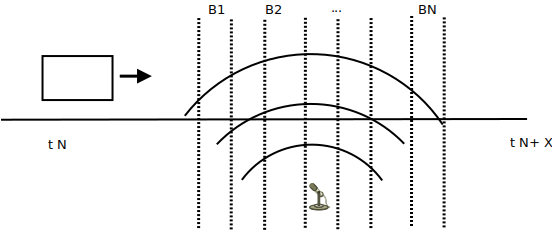
\includegraphics[scale=0.50]{../images/sound/soun_detect.png}
    \caption{Proceso de reconocimiento}
    \label{fig:recogn}
  \end{center}
\end{figure}

\newpage

\section{Almacenamiento de información}

La información será enviada desde los dispositivos recolectores hasta el servidor que contiene la base de datos de Apache Cassandra que se encontrará instalada en una instancia propia para garantizar que todos los recursos de la máquina se dedican a atender las peticiones de almacenamiento. Por otra parte las peticiones HTTP se realizarán mediante ficheros JSON contra una API Rest construida bajo Django-Rest-Framework

Ésta base de datos será de tipo NoSQL debido a que no se requiere ningún tipo de jerarquía sobre los datos y tampoco se precisa una estricta integridad de los mismos ni operaciones de tipo atómico.

\bigskip

Por otra parte tenemos la base de datos de la que hará uso la web de RSMap para la representación en el mapa. Al ser datos de caracter temporal cuyo formato no mantiene ningún tipo de jerarquía relacional se usará SQLite.

\section{Representación de información}

Éste módulo trabaja con Apache Zeppelin que también se encontrará en un servidor externo a los demás. En la configuración se establecerá la conexión hacia el servidor de almacenamiento masivo y a partir de ahí, se podrán lanzar consultas para obtener datos.

\newpage

\section{Diseño del portal web}

El portal estará desarrollao con el framework Django, el cual hace uso del paradigma modelo Vista-Controlador por lo que tendremos por una parte la parte lógica o Backend y por otro lado la parte visual o Frontend. Tendrá la siguiente estructura de archivos y directorios:

\begin{itemize}
  \item \textbf{resources}: archivos complementarios (no necesarios).
  \item \textbf{rsmap}: contiene el proyecto principal de la aplicación en el que se definen los parámetros generales.
  \begin{itemize}
      \item \textit{urls.py}: definicióno de las rutas globales de la web.
      \item \textit{wsgi.py}: configuración de despliegue.
      \item \textit{settings.py}: archivo de configuración general.
  \end{itemize}
  \item \textbf{rsmapweb}: contiene la aplicación web y la API rest.
  \begin{itemize}
    \item \textbf{templates}: contiene las plantillas html de la web.
    \begin{itemize}
      \item \textit{(index.html)} alberga la página principal.
      \item \textit{(map.html)} representa la página que contiene el mapa.
    \end{itemize}
    \item \textbf{static}: contiene los archivos estáticos de la web (css, fuentes, etc).
      \begin{itemize}
        \item \textbf{js}: es el directorio más importante ya que contiene el script encargado de interactuar con el mapa \textit{(rsmapMapUpdater.js)}
      \end{itemize}
    \item \textit{admin.py} archivo para configurar la administración del portal.
    \item \textit{apps.py}: archivo en el que se configura las aplicaciones instaladas de la web.
    \item \textit{models.py}: modelos de datos que serán usados.
    \item \textit{urls.py}: definicióno de las rutas de la aplicación y la API rest.
    \item \textit{serializers.py}: define qué información devolverá al API rest.
    \item \textit{views.py}: definición de vistas
  \end{itemize}
    \item \textit{manage.py}: encargado de ejecutar tareas de lanzar la aplicación además de actualizar los modelos de datos en la base de datos.
    \item \textit{requirements.txt}: dependencias necesarias para la aplicación.
    \item \textit{Makefile}: contiene la automatización de las tareas más comunes de la aplicación.
\end{itemize}

La API en JavaScript de Google Maps nos proporcionará las herramientas necesarias para generar y alimentar un mapa con la información que deseemos.

\bigskip

En lo que a la parte visual se refiere, se usará Bootstrap para garantizar un diseño adaptativo al formato de dispositivo desde el cual se consulte la información.

\subsection{Diseño de la api REST}

La api estará integrada dentro de Django gracias al módulo Django-Rest-Framework, es por éste motivo por lo que se desarrolla dentro de la sección \textit{Diseño del portal web}.

\bigskip

Una API se caracteriza por ofrecer una serie de URL's sobre las que realizar peticiones HTTP de diverso tipo como podrían ser POST, GET, PATCH, PUT o DELETE entre otras.

Éstas peticiones contienen un \textit{payload} con la información necesaria para que, una vez recibida la petición, la API se encarge internamente de interactuar con los modelos creados en Django que afecten a la misma.

\bigskip

Las rutas tendrán una estructura similar a la siguiente:

\begin{itemize}
  \item \textbf{Consultar listado o añadir dispositivos al mismo:}

  \url{http://urlweb/api/signals/}

  Devolverá un JSON con los dispositivos que están retransmitiendo información en ese momento (GET), además ésta ruta debe permitir registrar nuevos dispositivos (POST) por lo que los métodos permitidos en ella serán POST y GET.

  \item \textbf{Actualizar estado de dispositivo:}

  \url{http://urlweb/api/signal/signalID}

  Con ésta url podremos obtener los detalles de esta señal en concreto (GET), actualizar el estado de una señal (PATCH) o eliminarla en consecuencia de que el dispositivo deje de retransmitir (DELETE), de ésta manera el servidor web no tendrá que descargar continuamente el JSON de todos los dispositivos para representarlo en el mapa si no únicamente aquellos que se encuentren retransmitiendo en ese momento. Por tanto los métodos permitidos para ésta URL serán GET, PATCH y DELETE.
\end{itemize}
